\section{Evaluation}
\label{sec:classifiers-evaluation}

We now evaluate the effectiveness of using machine learning classifiers to predict energy-efficient system settings during application runtime.
First, we compare against the naive \emph{race-to-idle} heuristic, \ie all sockets allocated with HyperThreads and DVFS set to TurboBoost, and against a DVFS \emph{Oracle}.
We then quantify how varying sampling/prediction intervals and the number and types of features impacts classifier effectiveness.
We discuss how application dynamics affect the classifiers and evaluate the overhead of different parts of the classifier runtime.
Finally, we explore using separate classifiers for taskset and DVFS, then discuss limitations.


\subsection{Reducing Energy Consumption}
\label{sec:eval-first}

\begin{figure}[t]
  \centering
  \begin{tikzpicture}
\definecolor{s1}{RGB}{228, 26, 28}
\definecolor{s2}{RGB}{55, 126, 184}
\definecolor{s3}{RGB}{77, 175, 74}
\definecolor{s4}{RGB}{152, 78, 163}
\definecolor{s5}{RGB}{255, 127, 0}

\begin{groupplot}[
    group style={
        group name=plots,
        group size=1 by 1,
        xlabels at=edge bottom,
        xticklabels at=edge bottom,
        vertical sep=5pt
    },
% axis x line* = bottom,
xlabel near ticks,
major x tick style = transparent,
xlabel={},
height=3.5cm,
width=0.95\columnwidth,
xmin=0.5,
xmax=4.5,
enlargelimits=false,
tick align = outside,
tick style={white},
ylabel style={align=center},
ytick=\empty,
ymin=0.6,
ymax=1.1,
ytick={0,0.2,0.4,0.6,0.8,1.0,1.2},
yticklabels={0.0,0.2,0.4,0.6,0.8,1.0,1.2},
legend cell align=left, 
legend style={ column sep=1ex },
ymajorgrids,
grid style={dashed},
]

\nextgroupplot[ylabel={Energy \\ (Normalized)},
ybar=\pgflinewidth,
legend entries = {{ET},{GB},{KNN},{MLP},{SVM},{Oracle}},
legend style={draw=none,legend columns=6,at={(.5,1.4)},anchor=north},
bar width=8pt,
ylabel shift={0mm},
xticklabel shift={0pt},
x tick label style={rotate=35, anchor=east, font=\scriptsize},
xtick={1,2,3,4,5,6,7},
xticklabels={
{HipMer},
{IDBA},
{Megahit},
{metaSPAdes},
},
execute at end plot={
% "Race":
\draw[thin, dashed] (axis cs:\pgfkeysvalueof{/pgfplots/xmin},1) -- (axis cs:\pgfkeysvalueof{/pgfplots/xmax},1);
% "Best static DVFS":
% \draw[thick, dotted] (axis cs:\pgfkeysvalueof{/pgfplots/xmin},0.765646972) -- (axis cs:\pgfkeysvalueof{/pgfplots/xmax},0.765646972);
% hack to reset column line style (ghostscript seems to use last formatting as line style, e.g. dashed or dotted instead of solid)
\draw[thin, solid] (axis cs:\pgfkeysvalueof{/pgfplots/xmin},\pgfkeysvalueof{/pgfplots/ymin}) -- (axis cs:\pgfkeysvalueof{/pgfplots/xmax},\pgfkeysvalueof{/pgfplots/ymin});
},
]
\addplot table[x index=0,y index=2, col sep=tab] {img/classifiers/compare_apps_pca4.txt};
\addplot table[x index=0,y index=3, col sep=tab] {img/classifiers/compare_apps_pca4.txt};
\addplot table[x index=0,y index=4, col sep=tab] {img/classifiers/compare_apps_pca4.txt};
\addplot table[x index=0,y index=5, col sep=tab] {img/classifiers/compare_apps_pca4.txt};
\addplot table[x index=0,y index=6, col sep=tab] {img/classifiers/compare_apps_pca4.txt};
\addplot table[x index=0,y index=7, col sep=tab] {img/classifiers/compare_apps_pca4.txt};

\end{groupplot}

\end{tikzpicture}
  \caption{Average application energy consumption using four performance counters at 5 second prediction intervals (lower is better).}
  \label{fig:compare-apps-pca4}
  % \vskip -1.0em
\end{figure}

We first demonstrate how effective runtime classification is at reducing energy consumption.
\figref{compare-apps-pca4} demonstrates results for each application, normalized to the \emph{race-to-idle} setting (dashed line) for each.
On average across all four applications, energy consumption is reduced by 19.3\%.
The most extreme results are from the \app{IDBA} and \app{Megahit} applications.
For \app{IDBA}, each classifier outperforms the \emph{Oracle}---the average energy savings is 28.1\%, and as much as 30.2\% when using the GB classifier.
Conversely, for \app{Megahit}, the classifiers have the highest energy consumption over the \emph{Oracle}, though still always better than \emph{race-to-idle}.
\app{Megahit} saves 11\% energy on average---8.7\% in the worst case with ET, and 15\% at best with MLP.
The behavior for these applications is discussed further in \secref{eval-dynamics}.
% We note both here and in the remainder of the evaluation that there is no consistently best classifier across applications.

The \emph{Oracle} is the most energy-efficient statically-selected DVFS frequency using all sockets and HyperThreads, and it difficult to beat.
Computing the \emph{Oracle} requires expensive offline characterization to determine the best static setting for each application and its input/configuration, making it impractical to determine for most applications.
It also does not have any overhead except for running PCM in the background.
The \emph{Oracle} can only be beat when an application does not require its full taskset (socket and HyperThreads) allocation to run efficiently.
HPC applications are designed to parallelize well, meaning this is not the typical use case, but opportunities do occur, \eg during prolonged memory or I/O-intensive phases.

\begin{figure}[t]
% python ClassificationPlotUtils.py -s boggle -c boggle/characterizations/HIPMER/0xFFFFFFFFFFFFFFFFFFFFFFFFFFFFFFFFFFFFFFFF_2101000/pcm.csv boggle/classifications/5s/HIPMER_moredata/ET/pcm.csv -i 1 5
  \centering
  % \vskip -0.1em
  \subfloat[\app{HipMer} in naive static \emph{race-to-idle} heuristic.]
  % {\centering \includegraphics[width=\columnwidth]{figs/ts_hipmer_2101000_pca4.pdf}
  {\centering \begin{tikzpicture}

\definecolor{s1}{RGB}{228, 26, 28}
\definecolor{s2}{RGB}{55, 126, 184}
\definecolor{s3}{RGB}{77, 175, 74}
\definecolor{s4}{RGB}{152, 78, 163}
\definecolor{s5}{RGB}{255, 127, 0}

\begin{groupplot}[
    group style={
        group name=plots,
        group size=1 by 1,
        xlabels at=edge bottom,
        xticklabels at=edge bottom,
        vertical sep=5pt
    },
height=3.5cm,
width=0.95\columnwidth,
xmajorgrids,
ymajorgrids,
grid style={dashed},
xmin=0,
xmax=3465,
xtick={0,500,1000,1500,2000,2500,3000,3500},
ymin=0,
ymax=1.05,
ytick={0,0.2,0.4,0.6,0.8,1.0},
yticklabels={0,0.2,0.4,0.6,0.8,1.0},
yticklabel pos=left,
enlargelimits=false,
tick align = outside,
tick style={white},
xticklabel shift={-5pt},
yticklabel shift={-5pt},
ylabel shift={-2pt},
ylabel style={align=center},
legend cell align=left,
legend style={ column sep=1ex },
unbounded coords=jump,
]

\nextgroupplot[ylabel={},
yticklabel style={font=\footnotesize},
xlabel={\footnotesize $time$ [seconds]},
xlabel near ticks,
xticklabels={0,500,1000,1500,2000,2500,3000,3500},
xticklabel style={font=\footnotesize},
legend entries={{Power},{EE},{Cumulative~Energy}},
legend style={draw=none,at={(0.5,1.4)},anchor=north,legend columns=4,line width=5pt},
]
\addplot[thick, solid, color=s2] table[x index=0,y index=1,col sep=comma] {img/classifiers/ts_hipmer/ts_hipmer_2101000_pca4.csv};
\addplot[thick, solid, color=s3] table[x index=0,y index=2,col sep=comma] {img/classifiers/ts_hipmer/ts_hipmer_2101000_pca4.csv};
\addplot[thick, solid, color=s1] table[x index=0,y index=3,col sep=comma] {img/classifiers/ts_hipmer/ts_hipmer_2101000_pca4.csv};
\addplot[thin, solid, black] coordinates {(2206,0) (2206, 250)};

\end{groupplot}

\end{tikzpicture}
  \label{fig:ts-hipmer-dvfs}
  % \vspace{ -1.5em }
  }
  \\
  % \vskip -1.5em
  \subfloat[\app{HipMer} with ET classifier at 5 second intervals.]
  % {\centering \includegraphics[width=\columnwidth]{figs/ts_hipmer_et_pca4.pdf}
  {\centering \begin{tikzpicture}

\definecolor{s1}{RGB}{228, 26, 28}
\definecolor{s2}{RGB}{55, 126, 184}
\definecolor{s3}{RGB}{77, 175, 74}
\definecolor{s4}{RGB}{152, 78, 163}
\definecolor{s5}{RGB}{255, 127, 0}

\begin{groupplot}[
    group style={
        group name=plots,
        group size=1 by 1,
        xlabels at=edge bottom,
        xticklabels at=edge bottom,
        vertical sep=5pt
    },
height=3.5cm,
width=0.95\columnwidth,
xmajorgrids,
ymajorgrids,
grid style={dashed},
xmin=0,
xmax=3465,
xtick={0,500,1000,1500,2000,2500,3000,3500},
ymin=0,
ymax=1.05,
ytick={0,0.2,0.4,0.6,0.8,1.0},
yticklabels={0,0.2,0.4,0.6,0.8,1.0},
yticklabel pos=left,
enlargelimits=false,
tick align = outside,
tick style={white},
xticklabel shift={-5pt},
yticklabel shift={-5pt},
ylabel shift={-2pt},
ylabel style={align=center},
legend cell align=left,
legend style={ column sep=1ex },
unbounded coords=jump,
]

\nextgroupplot[ylabel={},
yticklabel style={font=\footnotesize},
xlabel={\footnotesize $time$ [seconds]},
xlabel near ticks,
xticklabels={0,500,1000,1500,2000,2500,3000,3500},
xticklabel style={font=\footnotesize},
legend entries={{Power},{EE},{Cumulative.~Energy}},
legend style={draw=none,at={(0.5,1.4)},anchor=north,legend columns=4,line width=5pt},
]
\addplot[thick, solid, color=s2] table[x index=0,y index=1,col sep=comma] {img/classifiers/ts_hipmer/ts_hipmer_et_pca4.csv};
\addplot[thick, solid, color=s3] table[x index=0,y index=2,col sep=comma] {img/classifiers/ts_hipmer/ts_hipmer_et_pca4.csv};
\addplot[thick, solid, color=s1] table[x index=0,y index=3,col sep=comma] {img/classifiers/ts_hipmer/ts_hipmer_et_pca4.csv};
\addplot[thin, solid, black] coordinates {(3465,0) (3465, 250)};

\end{groupplot}

\end{tikzpicture}
  \label{fig:ts-hipmer-all-et}
  % \vspace{ -1.5em }
  }
  \caption{Execution time, power, energy efficiency, and energy consumption behavior for the \app{HipMer} application (a) without and (b) with classification.}
  \label{fig:ts-hipmer}
  % \vskip -1.0em
\end{figure}

To demonstrate how energy savings are achieved, \figref{ts-hipmer} shows the runtime, power, energy efficiency, and cumulative energy consumption for executions of the \app{HipMer} application (Y values are normalized across both time series for each metric).
\figref{ts-hipmer-dvfs} runs \app{HipMer} in the \emph{race-to-idle} heuristic, and although the runtime is short, the high power also results in poor energy consumption.
In contrast, \figref{ts-hipmer-all-et} demonstrates running with the ET classifier---the execution takes longer, but the significantly lower power results in nearly 20\% less energy consumption in total, despite the increase in runtime.
Each figure shows clear phases in the execution, indicated by relatively long-term changes in both power and energy efficiency (per \eqnref{ee}, a function of instruction rate and power).
Classifiers adapt to changes in feature values like instruction rate and power by changing their predictions to run the application more efficiently, thus decreasing total energy consumption.


\subsection{Classifier Interval and Feature Selection}
\label{sec:eval-clf-settings}

\begin{figure}[t]
  \centering
  \begin{tikzpicture}
\definecolor{s1}{RGB}{228, 26, 28}
\definecolor{s2}{RGB}{55, 126, 184}
\definecolor{s3}{RGB}{77, 175, 74}
\definecolor{s4}{RGB}{152, 78, 163}
\definecolor{s5}{RGB}{255, 127, 0}

\begin{groupplot}[
    group style={
        group name=plots,
        group size=1 by 1,
        xlabels at=edge bottom,
        xticklabels at=edge bottom,
        vertical sep=5pt
    },
% axis x line* = bottom,
xlabel near ticks,
major x tick style = transparent,
xlabel={},
height=3.5cm,
width=0.95\columnwidth,
xmin=0.5,
xmax=5.5,
enlargelimits=false,
tick align = outside,
tick style={white},
ylabel style={align=center},
ytick=\empty,
ymin=0.6,
ymax=1.1,
ytick={0.6,0.7,0.8,0.9,1.0,1.1},
yticklabels={0.6,0.7,0.8,0.9,1.0,1.1},
legend cell align=left, 
legend style={ column sep=1ex },
ymajorgrids,
grid style={dashed},
]

\nextgroupplot[ylabel={Energy \\ (Normalized)},
ybar=\pgflinewidth,
legend entries = {{1~sec},{5~sec},{10~sec}},
legend style={draw=none,legend columns=5,at={(.5,1.4)},anchor=north},
bar width=8pt,
ylabel shift={0mm},
xticklabel shift={0pt},
x tick label style={rotate=35, anchor=east, font=\scriptsize},
xtick={1,2,3,4,5,6,7},
xticklabels={
{ET},
{GB},
{KNN},
{MLP},
{SVM},
},
execute at end plot={
% "Race":
\draw[thin, dashed] (axis cs:\pgfkeysvalueof{/pgfplots/xmin},1) -- (axis cs:\pgfkeysvalueof{/pgfplots/xmax},1);
% "Best static DVFS":
\draw[thick, dotted] (axis cs:\pgfkeysvalueof{/pgfplots/xmin},0.765646972) -- (axis cs:\pgfkeysvalueof{/pgfplots/xmax},0.765646972);
% hack to reset column line style (ghostscript seems to use last formatting as line style, e.g. dashed or dotted instead of solid)
\draw[thin, solid] (axis cs:\pgfkeysvalueof{/pgfplots/xmin},\pgfkeysvalueof{/pgfplots/ymin}) -- (axis cs:\pgfkeysvalueof{/pgfplots/xmax},\pgfkeysvalueof{/pgfplots/ymin});
},
]
\addplot table[x index=0,y index=7, col sep=tab] {img/classifiers/compare_interval/compare_1s.txt};
\addplot table[x index=0,y index=7, col sep=tab] {img/classifiers/compare_interval/compare_5s.txt};
\addplot table[x index=0,y index=7, col sep=tab] {img/classifiers/compare_interval/compare_10s.txt};

\end{groupplot}

\end{tikzpicture}
  \caption{Average energy consumption for different sampling/prediction intervals (lower is better).}
  \label{fig:interval}
  % \vskip -1.0em
\end{figure}

There are a variety classifier settings to configure at runtime.
This section evaluates the classifiers' ability to reduce energy consumption by varying prediction interval and the number and types of features used.

The sampling and prediction interval dictates how quickly a classifier can respond to changes in application behavior, but also incurs overhead and affects a classifier's susceptibility to noise.
\figref{interval} shows the normalized energy consumption, averaged across applications, for each classifier at 1, 5, and 10 second intervals.
The thin dotted line at 0.75 is the average normalized energy consumption for the \emph{Oracle}.
The 1 second interval is clearly the worst, only outperforming the others for the ET classifier.
It is closer to the \emph{race-to-idle} heuristic than the \emph{Oracle} for GB and SVM, but still better than \emph{race-to-idle}.
Both the 5 and 10 second intervals perform well---although the 10 second interval does better for one particular classifier (KNN), the 5 second interval is similar on average and is more responsive.
We elect to use the 5 second interval for the remainder of our experiments, as it provides a good tradeoff of energy efficiency and responsiveness to changing application behavior.

\begin{figure}[t]
  \centering
  % \vskip -0.1em
  \subfloat[Average energy consumption based on number of features.]
  {\centering \begin{tikzpicture}
\definecolor{s1}{RGB}{228, 26, 28}
\definecolor{s2}{RGB}{55, 126, 184}
\definecolor{s3}{RGB}{77, 175, 74}
\definecolor{s4}{RGB}{152, 78, 163}
\definecolor{s5}{RGB}{255, 127, 0}

\begin{groupplot}[
    group style={
        group name=plots,
        group size=1 by 1,
        xlabels at=edge bottom,
        xticklabels at=edge bottom,
        vertical sep=5pt
    },
% axis x line* = bottom,
xlabel near ticks,
major x tick style = transparent,
xlabel={},
height=3.5cm,
width=0.95\columnwidth,
xmin=0.5,
xmax=5.5,
enlargelimits=false,
tick align = outside,
tick style={white},
ylabel style={align=center},
ytick=\empty,
ymin=0.6,
ymax=1.1,
ytick={0.6,0.7,0.8,0.9,1.0,1.1},
yticklabels={0.6,0.7,0.8,0.9,1.0,1.1},
legend cell align=left, 
legend style={ column sep=1ex },
ymajorgrids,
grid style={dashed},
]

\nextgroupplot[ylabel={Energy \\ (Normalized)},
ybar=\pgflinewidth,
legend entries = {{One},{Two},{Three},{Four},{Five},{All}},
legend style={draw=none,legend columns=6,at={(.5,1.4)},anchor=north},
bar width=8pt,
ylabel shift={0mm},
xticklabel shift={0pt},
x tick label style={rotate=35, anchor=east, font=\scriptsize},
xtick={1,2,3,4,5,6,7},
xticklabels={
{ET},
{GB},
{KNN},
{MLP},
{SVM},
},
execute at end plot={
% "Race":
\draw[thin, dashed] (axis cs:\pgfkeysvalueof{/pgfplots/xmin},1) -- (axis cs:\pgfkeysvalueof{/pgfplots/xmax},1);
% "Best static DVFS":
\draw[thick, dotted] (axis cs:\pgfkeysvalueof{/pgfplots/xmin},0.765646972) -- (axis cs:\pgfkeysvalueof{/pgfplots/xmax},0.765646972);
% hack to reset column line style (ghostscript seems to use last formatting as line style, e.g. dashed or dotted instead of solid)
\draw[thin, solid] (axis cs:\pgfkeysvalueof{/pgfplots/xmin},\pgfkeysvalueof{/pgfplots/ymin}) -- (axis cs:\pgfkeysvalueof{/pgfplots/xmax},\pgfkeysvalueof{/pgfplots/ymin});
},
]
\addplot table[x index=0,y index=7, col sep=tab] {img/classifiers/compare_pca/pca1.txt};
\addplot table[x index=0,y index=7, col sep=tab] {img/classifiers/compare_pca/pca2.txt};
\addplot table[x index=0,y index=7, col sep=tab] {img/classifiers/compare_pca/pca3.txt};
\addplot table[x index=0,y index=7, col sep=tab] {img/classifiers/compare_pca/pca4.txt};
\addplot table[x index=0,y index=7, col sep=tab] {img/classifiers/compare_pca/pca5.txt};
\addplot table[x index=0,y index=7, col sep=tab] {img/classifiers/compare_interval/compare_5s.txt};

\end{groupplot}

\end{tikzpicture}
  \label{fig:compare-pca}
  % \vspace{ -1.5em }
  }
  \\
  % \vskip -1.5em
  \subfloat[Average energy consumption based on types of features.]
  {\centering \begin{tikzpicture}
\definecolor{s1}{RGB}{228, 26, 28}
\definecolor{s2}{RGB}{55, 126, 184}
\definecolor{s3}{RGB}{77, 175, 74}
\definecolor{s4}{RGB}{152, 78, 163}
\definecolor{s5}{RGB}{255, 127, 0}

\begin{groupplot}[
    group style={
        group name=plots,
        group size=1 by 1,
        xlabels at=edge bottom,
        xticklabels at=edge bottom,
        vertical sep=5pt
    },
% axis x line* = bottom,
xlabel near ticks,
major x tick style = transparent,
xlabel={},
height=3.5cm,
width=0.95\columnwidth,
xmin=0.5,
xmax=5.5,
enlargelimits=false,
tick align = outside,
tick style={white},
ylabel style={align=center},
ytick=\empty,
ymin=0.6,
ymax=1.1,
ytick={0,0.2,0.4,0.6,0.8,1.0,1.2},
yticklabels={0.0,0.2,0.4,0.6,0.8,1.0,1.2},
legend cell align=left, 
legend style={ column sep=1ex },
ymajorgrids,
grid style={dashed},
]

\nextgroupplot[ylabel={Energy \\ (Normalized)},
ybar=\pgflinewidth,
legend entries = {{All},{NoPower},{NoDramTotalExec}},
legend style={draw=none,legend columns=4,at={(.5,1.4)},anchor=north},
bar width=8pt,
ylabel shift={0mm},
xticklabel shift={0pt},
x tick label style={rotate=35, anchor=east, font=\scriptsize},
xtick={1,2,3,4,5,6,7},
xticklabels={
{ET},
{GB},
{KNN},
{MLP},
{SVM},
},
execute at end plot={
% "Race":
\draw[thin, dashed] (axis cs:\pgfkeysvalueof{/pgfplots/xmin},1) -- (axis cs:\pgfkeysvalueof{/pgfplots/xmax},1);
% "Best static DVFS":
\draw[thick, dotted] (axis cs:\pgfkeysvalueof{/pgfplots/xmin},0.765646972) -- (axis cs:\pgfkeysvalueof{/pgfplots/xmax},0.765646972);
% hack to reset column line style (ghostscript seems to use last formatting as line style, e.g. dashed or dotted instead of solid)
\draw[thin, solid] (axis cs:\pgfkeysvalueof{/pgfplots/xmin},\pgfkeysvalueof{/pgfplots/ymin}) -- (axis cs:\pgfkeysvalueof{/pgfplots/xmax},\pgfkeysvalueof{/pgfplots/ymin});
},
]

\addplot table[x index=0,y index=7, col sep=tab] {img/classifiers/compare_interval/compare_5s.txt};
\addplot table[x index=0,y index=7, col sep=tab] {img/classifiers/compare_pca/pca_nopower.txt};
\addplot table[x index=0,y index=7, col sep=tab] {img/classifiers/compare_pca/pca_nodramtotalexec.txt};

\end{groupplot}

\end{tikzpicture}
  \label{fig:compare-robustness}
  % \vspace{ -1.5em }
}
  \caption{Average energy consumption, varying the number and types of available features (lower is better).}
  \label{fig:pca}
  % \vskip -1.0em
\end{figure}

In \figref{pca-evr} (\secref{setup-training}) we quantified the variation contribution of different features (performance counters).
Now we evaluate how varying the features impacts classifier behavior, since the number and types of features contribute to runtime complexity and prediction accuracy.
We run with 5 second sampling/prediction intervals and present the results in \figref{pca}.

\figref{compare-pca} varies the number of features used.
\pc{POWER\_DRAM} is the only feature used for $One$, \pc{POWER\_DRAM} and \pc{EXEC} are used for $Two$, etc.
For $All$, all 16 features are used.
Using a single feature works surprisingly well for most classifiers, but performs poorly with KNN, which too often predicts settings that use only a single socket.
It is a little surprising that a single feature can be so effective otherwise, but \pc{POWER\_DRAM} does account for 42\% of the explained variance, and is correlated with other performance counters like cache hit and miss rates.
Using two or three features also works quite well, but four features is the best for most classifiers, accounting for 84\% of the variance.
The $Four$ configuration was previously broken down by application in \secref{eval-first}.

\figref{compare-robustness} selectively removes available features.
$NoPower$ drops the \pc{POWER\_DRAM}, \pc{POWER\_Proc}, and \pc{POWER\_Total} features.
This is a particularly important scenario, as not all systems have power/energy counters available at runtime.
When all three power-related features are ignored, \pc{L3MISS\_Rate} is used as the first feature, and \pc{EXEC} remains the second.
(If \pc{POWER\_DRAM} is excluded exclusively, \pc{POWER\_Total} becomes the primary feature instead.)
Offline analysis also shows that \pc{READ\_Rate} can be used as the primary feature, depending on the exact training data.
$NoDramTotalExec$ drops \pc{POWER\_DRAM}, \pc{POWER\_Total}, and \pc{EXEC}, making \pc{AFREQ} and \pc{WRITE\_Rate} the primary and secondary features.
In general, $All$ outperforms the other two, but $NoPower$ does slightly better for the ET classifier, as does $NoDramTotalExec$ with MLP.
None of the configurations perform poorly, demonstrating that the classification approach is robust to different numbers and types of features.


\subsection{Application Dynamics}
\label{sec:eval-dynamics}

The results thus far raise the question: why does the \emph{Oracle} often perform better than the classifiers?
First, we recall that the \emph{Oracle} requires each application to be characterized across all DVFS settings with their current input and configuration, so is not practical to discover for most applications in practice.
Additionally, the \emph{Oracle} does not incur any overhead except sampling PCM (runtime overheads are quantified next in \secref{classifiers-eval-overhead}), and can only be beat when applications do not require all sockets and HyperThreads.
In fact, for 3 of the 4 evaluation applications, classification usually achieves energy consumption close to that of the \emph{Oracle}, and sometimes better.

Energy consumption penalties are incurred primarily by two factors: 1) overhead from changing settings, and 2) running in inefficient settings.
While there is no particular threshold for determining when changes to performance counter values result in a new prediction, we quantify the difficulty in controlling applications by examining performance counters' coefficients of variation during the course of an application execution.
Since applications move through phases, a high coefficient of variation for an execution does not cause problems on its own.
The difficulty arises when performance counter values fluctuate rapidly enough to cause the classifiers to predict new system settings, constantly incurring actuation overhead and spending time in suboptimal settings.

\begin{figure}[t]
  \centering
  \begin{tikzpicture}

\definecolor{s1}{RGB}{228, 26, 28}
\definecolor{s2}{RGB}{55, 126, 184}
\definecolor{s3}{RGB}{77, 175, 74}
\definecolor{s4}{RGB}{152, 78, 163}
\definecolor{s5}{RGB}{255, 127, 0}

\begin{groupplot}[
    group style={
        group name=plots,
        group size=1 by 2,
        xlabels at=edge bottom,
        xticklabels at=edge bottom,
        vertical sep=5pt
    },
height=3.5cm,
width=\columnwidth,
xmajorgrids,
ymajorgrids,
grid style={dashed},
xmin=0,
xmax=600,
yticklabel pos=left,
enlargelimits=false,
tick align = outside,
tick style={white},
xticklabel shift={-5pt},
yticklabel shift={-5pt},
ylabel shift={-2pt},
ylabel style={align=center},
legend cell align=left,
legend style={ column sep=1ex },
unbounded coords=jump,
]

\nextgroupplot[ylabel={IDBA \\ Coeff. of Var.},
ytick={0,0.5,1.0,1.5,2.0},
yticklabels={,0.5,1.0,1.5,2.0},
yticklabel style={font=\footnotesize},
ymin=0,
ymax=2,
% xlabel={\footnotesize Time (s)},
xlabel near ticks,
xtick={0,100,200,300,400,500,600},
% xticklabels={0,100,200,300,400,500,600},
xticklabel style={font=\footnotesize},
legend entries={{POWER\_DRAM},{EXEC}},
legend style={draw=none,at={(0.5,1.4)},anchor=north,legend columns=4,line width=5pt},
]
\addplot[thick, solid, color=s1] table[x index=0,y index=2,col sep=tab] {img/classifiers/cv/coev_idba.txt};
\addplot[thick, solid, color=s2] table[x index=0,y index=1,col sep=tab] {img/classifiers/cv/coev_idba.txt};


\nextgroupplot[ylabel={Megahit \\ Coeff. of Var.},
ytick={0,0.5,1.0,1.5,2.0},
yticklabels={0,0.5,1.0,1.5,2.0},
yticklabel style={font=\footnotesize},
ymin=0,
ymax=2,
xlabel={\footnotesize $time$ [seconds]},
xlabel near ticks,
xtick={0,100,200,300,400,500,600},
xticklabels={0,100,200,300,400,500,600},
xticklabel style={font=\footnotesize},
]
\addplot[thick, solid, color=s1] table[x index=0,y index=2,col sep=tab] {img/classifiers/cv/coev_megahit.txt};
\addplot[thick, solid, color=s2] table[x index=0,y index=1,col sep=tab] {img/classifiers/cv/coev_megahit.txt};

\end{groupplot}

\end{tikzpicture}
  \caption{Runtime coefficient of variation over a 5 second sliding window (lower values indicates more stable application behavior).}
  \label{fig:cv}
  % \vskip -1.0em
\end{figure}

% Actuation overhead limits how frequently settings can reasonably be changed (observed in \secref{eval-clf-settings} and quantified next in \secref{classifiers-eval-overhead}).
% Even so, a very real penalty is also incurred when new settings turn out not to be energy-efficient due to the application rapidly changing its behavior before another prediction is made and actuated.
In \figref{cv}, we examine \pc{POWER\_DRAM} and \pc{EXEC} performance counter behaviors without any runtime actuation, with all sockets/cores allocated and using the maximum DVFS frequency without TurboBoost (to avoid fluctuations incurred when temporarily running in higher DVFS frequencies).
For the first 10 minutes of each execution, we compute coefficient of variation over 5 second windows to demonstrate the variability that our classifiers see.
We present results for \app{IDBA}, which in most cases outperforms the \emph{Oracle}, and for \app{Megahit}, which exhibits rapid fluctuations and consistently performs worse than the \emph{Oracle} (but still better than \emph{race-to-idle}).
While \app{IDBA} does exhibit fluctuations, they are typically short-lived---most of the time the performance counter values are relatively stable.
In contrast, \app{Megahit} is constantly noisy, resulting in frequent changes to system settings.

\begin{table}[t]
\caption{Frequency of settings changes for ET classifier in the $All$ configuration.}
\label{tbl:classifiers-actuation}
\small
\centering
\begin{tabular}{c|c|c|c}
  \textbf{Application} & \textbf{Prediction} & \textbf{Taskset} & \textbf{DVFS} \\
  \hline
  HipMer     & 32.7\% & 25.6\% & 23.1\% \\
  IDBA       & 39.9\% & 37.4\% & 18.8\% \\
  Megahit    & 46.6\% & 37.9\% & 39.8\% \\
  metaSPAdes & 41.9\% & 32.9\% & 28.6\% \\
  \hline
\end{tabular}
% \vskip -.7em
\end{table}

For example, \tblref{classifiers-actuation} quantifies how frequently predictions and system settings change when using the ET classifier in the $All$ configuration.
\app{Megahit} has the highest frequency of changing predictions, but more importantly (and difficult to quantify), is how extreme the fluctuations' impacts	 are.
With \app{IDBA}, the classifier prefers to switch between one socket and four sockets, always with HyperThreads enabled; DVFS is typically around 1.8 GHz, other times running in TurboBoost.
With \app{Megahit}, the classifier chooses four sockets with HyperThreads, four sockets without HyperThreads, and one socket with HyperThreads; DVFS is consistently around 1.7 or 1.8 GHz, periodically running in TurboBoost when all cores also being used.
\app{Megahit} also poses an additional technical challenge---it appears to constantly destroy and spawn threads, which sometimes makes managing its taskset difficult.

In short, the dynamic behavior that applications exhibit can make predicting energy-efficient settings at runtime a challenge.
Handling variability is not something the classifiers learn during training.
However, any resource management system that is dependent on runtime feedback must find a good balance between responsiveness and susceptibility to noisy data---a challenge not limited to using classification.
% For practical purposes, a fielded solution might address this problem by applying smoothing or other noise reduction techniques to the performance counter data.


\subsection{Overhead}
\label{sec:classifiers-eval-overhead}

For classification to be practical, the runtime overhead must be reasonable.
This section quantifies the overhead of different components/stages of the classification pipeline.

\begin{table}[th]
\caption{Classification runtime overheads.}
\label{tbl:classifiers-overhead}
\small
\centering
\begin{tabular}{c|c}
  \textbf{Stage} & \textbf{Average Overhead (ms)} \\
  \hline
  \hline
  Init -- Scaling/PCA & 4.50 \\
  Init -- ET          & 29.01 \\
  Init -- GB          & 3456.34 \\
  Init -- KNN         & 3.50 \\
  Init -- MLP         & 1278.30 \\
  Init -- SVM         & 68.92 \\
  \hline
  PCM Sampling        & 14.70 \\
  Scaling/PCA         & 0.08 \\
  Predict -- ET       & 0.75 \\
  Predict -- GB       & 0.36 \\
  Predict -- KNN      & 0.39 \\
  Predict -- MLP      & 0.14 \\
  Predict -- SVM      & 0.13 \\
  % \hline
  Actuation & $\approx 100$ \\
  \hline
  \hline
\end{tabular}
% \vskip -.7em
\end{table}

\tblref{classifiers-overhead} breaks down the runtime overhead on our evaluation system.
First, the data transformation (Scaling/PCA) and classifier must be initialized.
Initialization incurs the highest overhead, but of course only needs to be performed once and is trivial compared to total application runtime.
All classifiers we evaluated initialize within a few seconds, and some are much faster, initializing within a few dozen milliseconds.

To estimate the overhead incurred by reading the performance counters (PCM Sampling), we configure PCM to poll counters 1000 times at an interval that is faster than achievable (so it does not wait between reads), and time the execution.
As a result, the average value for PCM also accounts for its initialization and teardown time.

Transforming the PCM data (Scaling/PCA) prior to running the classifier is extremely fast, averaging about 80\us.
Prediction overheads vary by classifier, but the average overheads for each are strictly less than 1\ms.
The actuation overhead, while high compared to sampling and prediction, is a task that any runtime resource allocator that manages DVFS and taskset has to incur.
Although dependent on application behavior, in half to three-fourths of cases we find that no actuation overhead is incurred since the classifier's prediction does not change at each sampling interval (\tblref{classifiers-actuation}).
When there is a change, the overhead is on the order of 100\ms, which is consistent with observations on other server-class systems \cite{POETMCSoC}.

It is also import to note that PCM, the classifier, and the actuator run in parallel with the application under control, so the application does not stop making progress while the resource management components work.

As mentioned previously, we have not attempted to optimize any of these overhead results.
We expect that it is readily possible to reduce overhead, particularly in reading performance counters (PCM samples more performance counters than we actually use) and integrating with other tools for managing taskset \cite{Sridharan2013}.
Additionally, if initialization time is a concern, classifier state could be stored and reloaded between executions, or the classifier could just run continuously on the system.


\subsection{Using Separate Classifiers}
\label{sec:eval-separate-classifiers}

Our analysis thus far has used a single classifier to predict a label that is a combination of both taskset (socket allocation, including HyperThreads) and the DVFS frequency (including TurboBoost).
With 8 taskset options and 11 DVFS settings, there are 88 total possible labels for the classifier to choose from.
After labeling the training data, only a subset of these 88 will actually be used, but the size of that subset could increase with additional training data.

\begin{figure}[t]
  % \vskip -1.0em
  \centering
  \subfloat[Taskset only, recall=0.869.]
  {\centering 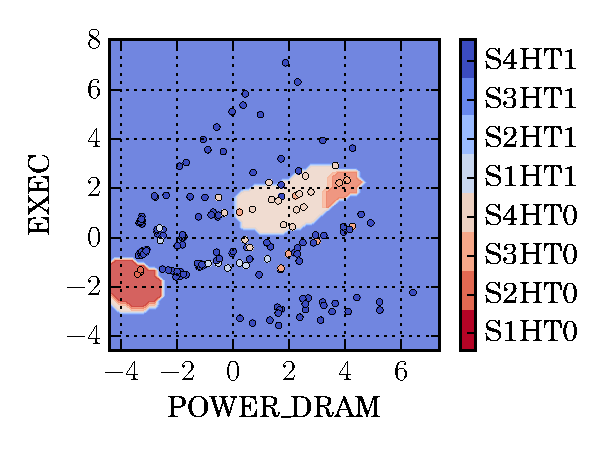
\includegraphics[width=0.3\columnwidth]{figs/classifiers/training_space_svm_ts.pdf}
  \label{fig:feat-svm-ts}
  % \vspace{ -1.5em }
  }
  % \\
  % \vskip -1.5em
  \hspace*{0.1cm}
  \subfloat[DVFS only, recall=0.645.]
  {\centering 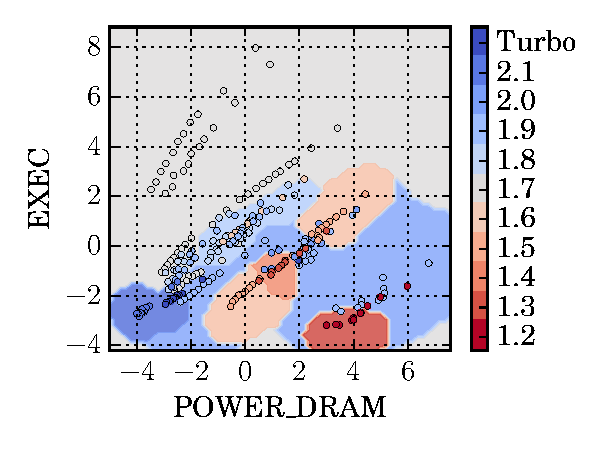
\includegraphics[width=0.3\columnwidth]{figs/classifiers/training_space_svm_dvfs.pdf}
  \label{fig:feat-space-svm-dvfs}
  % \vspace{ -1.5em }
}
\caption{Training data and learned decision boundaries for SVM when classifying for taskset and DVFS separately.}
\label{fig:feat-space-svm-separate}
% \vskip -1.0em
\end{figure}

An alternative approach is for one classifier to predict the taskset, and a separate classifier to predict the DVFS frequency.
\figref{feat-space-svm-separate} visualizes the training and recall for SVM (like \figref{feat-space-svm} in \secref{challenges-learning}) using separate classifiers.
Note that there are fewer data points, as DVFS is fixed at TurboBoost when training for taskset, and taskset is fixed at all sockets and HyperThreads when training for DVFS.
Taskset's recall is quite good, while DVFS is not as good as before.
There is, of course, additional overhead in running two classifiers instead of one, but \secref{classifiers-eval-overhead} demonstrated that data processing overhead is not significant, and there is still only a single instance of PCM and the actuators running.

\begin{figure}[t]
  \centering
  \begin{tikzpicture}
\definecolor{s1}{RGB}{228, 26, 28}
\definecolor{s2}{RGB}{55, 126, 184}
\definecolor{s3}{RGB}{77, 175, 74}
\definecolor{s4}{RGB}{152, 78, 163}
\definecolor{s5}{RGB}{255, 127, 0}

\begin{groupplot}[
    group style={
        group name=plots,
        group size=1 by 1,
        xlabels at=edge bottom,
        xticklabels at=edge bottom,
        vertical sep=5pt
    },
% axis x line* = bottom,
xlabel near ticks,
major x tick style = transparent,
xlabel={},
height=3.5cm,
width=0.95\columnwidth,
xmin=0.5,
xmax=5.5,
enlargelimits=false,
tick align = outside,
tick style={white},
ylabel style={align=center},
ytick=\empty,
ymin=0.6,
ymax=1.1,
ytick={0.6,0.7,0.8,0.9,1.0,1.1},
yticklabels={0.6,0.7,0.8,0.9,1.0,1.1},
legend cell align=left, 
legend style={ column sep=1ex },
ymajorgrids,
grid style={dashed},
]

\nextgroupplot[ylabel={Energy \\ (Normalized)},
ybar=\pgflinewidth,
legend entries = {{Single},{Separate}},
legend style={draw=none,legend columns=5,at={(.5,1.4)},anchor=north},
bar width=8pt,
ylabel shift={0mm},
xticklabel shift={0pt},
x tick label style={rotate=35, anchor=east, font=\scriptsize},
xtick={1,2,3,4,5,6,7},
xticklabels={
{ET},
{GB},
{KNN},
{MLP},
{SVM},
},
execute at end plot={
% "Race":
\draw[thin, dashed] (axis cs:\pgfkeysvalueof{/pgfplots/xmin},1) -- (axis cs:\pgfkeysvalueof{/pgfplots/xmax},1);
% "Best static DVFS":
\draw[thick, dotted] (axis cs:\pgfkeysvalueof{/pgfplots/xmin},0.765646972) -- (axis cs:\pgfkeysvalueof{/pgfplots/xmax},0.765646972);
% "ET_SVM"
\draw[thin, solid] (axis cs:\pgfkeysvalueof{/pgfplots/xmin},0.8288250669) -- (axis cs:\pgfkeysvalueof{/pgfplots/xmax},0.8288250669);
% hack to reset column line style (ghostscript seems to use last formatting as line style, e.g. dashed or dotted instead of solid)
\draw[thin, solid] (axis cs:\pgfkeysvalueof{/pgfplots/xmin},\pgfkeysvalueof{/pgfplots/ymin}) -- (axis cs:\pgfkeysvalueof{/pgfplots/xmax},\pgfkeysvalueof{/pgfplots/ymin});
},
]
\addplot table[x index=0,y index=7, col sep=tab] {img/classifiers/compare_interval/compare_5s.txt};
\addplot table[x index=0,y index=7, col sep=tab] {img/classifiers/compare_pca/sep_clfs.txt};

\end{groupplot}

\end{tikzpicture}
  \caption{Average energy consumption when using a single or separate classifiers for system knobs (lower is better).}
  \label{fig:separate-clfs}
  % \vskip -1.0em
\end{figure}

\figref{separate-clfs} quantifies the behavior when we use two separate classifiers simultaneously.
In each case, the same type of classifier is used for both taskset and DVFS prediction.
In three of five cases, $Separate$ actually outperforms the $Single$ approach.
However, it is also possible for $Separate$ to perform rather poorly, as seen with the MLP classifier.
The average MLP behavior is representative of the applications tested, \ie not caused by an outlier---in three of the four applications evaluated, MLP classifying taskset and DVFS separately performed worse than the \emph{race-to-idle} heuristic.
Of course, taskset and DVFS prediction may benefit from using different classification algorithms.
We tested taskset-only and DVFS-only classifiers in isolation and empirically determined that, for our system and applications, the ET classifier works best for taskset prediction and the SVM classifier works best for DVFS prediction.
The solid horizontal line indicates the energy consumption for this ET/SVM classifier mix.
While this avoided the poor results seen with MLP, it actually performed slightly worse than three of the four remaining $Single$ classifier approaches.
Using a single, unified classifier that learns both taskset and DVFS together ultimately produces more reliable predictions.


\subsection{Discussion of Results and Limitations}
\label{sec:eval-discuss}

Our evaluation demonstrates that machine learning classification driven by low-level features is an effective approach for improving energy efficiency.
In fact, a variety of different classifiers are useful for predicting energy-efficient system settings at runtime, even without classifier tuning.
No single classifier appears to have a clear advantage over others, though future work on fine-tuning the training data and classifiers, combined with evaluations on other platforms, may eventually produce a near-optimal implementation.

We also did not attempt to optimize the runtime's overhead---reading performance counters, data transformations, or system actuation.
Although low, there is still room for improvement, which could support faster sampling and prediction intervals and further improve energy consumption.

We currently only manage socket/core allocation at system-level.
Because applications are launched with a fixed number of threads, those threads are forced to share compute cores when we bind applications to fewer sockets or disable HyperThreads during runtime.
This over-subscription is usually not as efficient as matching the thread count to the available cores, \eg running 80 threads on our 80 physical cores is more efficient that binding 160 threads to those 80 cores.
Integration with application-level parallelism can further improve energy efficiency and reduce resource contention when binding applications to smaller tasksets \cite{Sridharan2013}.
% \TODO{Anything on memory allocation/interleaving? We really don't have a solution to this problem when using dynamic taskset.}

On large systems such as our evaluation platform, the processor and DRAM consume the majority of system power, which we are able to measure \cite{RAPL,PCMGit}.
There are other components like hard disks and network interfaces that are not currently accounted for.
While it is not common practice to instrument these other components for power/energy monitoring, such feedback could help resource management solutions achieve better total energy efficiency.
